\documentclass[a4paper,11pt]{article}





\RequirePackage{emoji} % Emoji support in (Lua)LaTeX. requires the LuaHBTeX engine. adding emojis
\usepackage[
    year=2025,
    title={MATH 71.1\\ \textsf{Ch.2 SALT \emoji{salt}\\ (Stopped from Appearing in the Long Test)}},
    shorttitle={SALT},
    problemlead={Problem},
    % bgimage={img/auxl/NOI2024pages.png},
    toclinkcolor=Goldenrod,
    boxtextcolor=black,
    boxbgcolor=AlgolympicsOrange2024
]{problemstatements}
\usepackage{CJKutf8}
\usepackage{fancyvrb}


\title{\contesttitle}
\date{October 22, 2025}


\begin{document}

\maketitle

\providecommand{\titlepagecoverimg}{img/auxl/cover.png}

\providecommand{\prefacenotesIO}{}
\providecommand{\prefacenotesinteractive}{}
\providecommand{\prefacenotesadditional}{}

% add this as \prefacenotesIO for finals
% We recommend learning and using these functions during the Practice Session.

% possible item to add, \prefacenotesadditional
% \item All problems are solvable in C++, but the same is not guaranteed for Python due to its slowness.



%%%%%%%%%%%%%%%%%%%%%%%%%%%%%%%%%%%%%%%%%%%%%%%%%%%%%%%%%
% title page
%%%%%%%%%%%%%%%%%%%%%%%%%%%%%%%%%%%%%%%%%%%%%%%%%%%%%%%%%






%%%%%%%%%%%%%%%%%%%%%%%%%%%%%%%%%%%%%%%%%%%%%%%%%%%%%%%%%
% long notes
%%%%%%%%%%%%%%%%%%%%%%%%%%%%%%%%%%%%%%%%%%%%%%%%%%%%%%%%%

% \newcommand\preem{rage}
\newcommand\preem{smiling-face-with-sunglasses}

\cleardoublepage

\markboth{Important!}{}
% \vspace*{0.05in}
% {\Large \color{red}{\textbf{Important!} Read the following:}}
% {\Huge {\color{red}{\textbf{Important!} Read the following: {\fontsize{80}{96}\texttt{\emoji{\preem}}} }} }
% {\Huge {\color{red}{\textbf{{\texttt{\emoji{rage}} Important!}} Read the following: }} }

% \newlength{\ragewidth}
% \newlength{\rageheight}
% \settowidth{\ragewidth}{\scalebox{3.3}{\texttt{\emoji{\preem}}}}
% \settoheight{\rageheight}{\texttt{\emoji{\preem}}}
% {\Huge{\color{red}{\textbf{%
%     % \makebox[\ragewidth][r]{\scalebox{2}{\texttt{\emoji{\preem}}}}
%     \parbox[b][\rageheight]{\ragewidth}{
%         \makebox[\ragewidth][r]{
%         \lapbox[\width]{17pt}{\raisebox{2pt}{\scalebox{5.2}{\texttt{\emoji{\preem}}}}}}}
%     Important!} Read the following:}}}

\textbf{Access the contest website} at the following url:
\begin{center}
    \url{TODO}
\end{center}
\bigskip

\begin{description}


%\item[Test Cases.]
\item[Hidden Test Cases.]
Your solution will be checked by running it against one or more (usually several) hidden test cases. \textbf{You will not have access to these cases}, but a correct solution is expected to handle them correctly. \\

% \item[Output Format.]
\item[Not Sorted by Difficulty.] The problem set is \textbf{not} sorted by difficulty!  Each team is encouraged to have at least read all the problems by the end of the contest. \\

\item[Submit Code Only.]
Only include \textbf{one} file when submitting: the source code (.py) and nothing else. \\

\item[Only Builtin Libraries.]
Do not use third-party libraries. Only libraries that come installed with the compilers are available on the evaluation machines. \\

% \item[Filename.]
\item[No Weird Filenames.]
Only use letters, digits and underscores in your filename. Do not use spaces or other special symbols. \\

\prefacenotesIO{}

% \item[Interactive Problems.]
% \item[Flush On Interactive Problems.]
% On interactive problems, make sure to \textbf{flush} your output stream after printing.
% \begin{itemize}
%     % weird hack with mintinline since it's converting << to a special character. feel free to use better fix
%     \item In C++, use \cpp{fflush(stdout);} or \mintinline[escapeinside=||]{cpp}{cout <||< endl;}
%     \item In Python, use \python{sys.stdout.flush()} or \python{print(flush=True)}
%     \item For more details, including for other languages, ask a question/clarification through CMS.
% \end{itemize}

% \prefacenotesinteractive{}

% \prefacenotesadditional{}

\end{description}

Good luck and enjoy the contest!  \texttt{\emoji{smiley}}


% TODO
% "how compprog works"
%     link to absolute beginner tutorial (video?), 
%     link to absolute beginner tutorial in abakoda?
%     link to absolute beginner tutorial document of our own making
% link to more specific/obscure/technical stuff (like java package name)
% link to verdicts page ("Documentation" in CMS)







%%%%%%%%%%%%%%%%%%%%%%%%%%%%%%%%%%%%%%%%%%%%%%%%%%%%%%%%%
% table of contents, and short notes
%%%%%%%%%%%%%%%%%%%%%%%%%%%%%%%%%%%%%%%%%%%%%%%%%%%%%%%%%

\setBG{\contestbg}

% \textsf{\tableofcontents}
% \markboth{Table of Contents}{}

% \begin{comment}
% \section*{Notes}

% these notes are intentionally repeated from the "Very Important" section below.

% \begin{itemize}
% \item Many problems have large input file sizes, so use fast I/O. For example:
% \begin{itemize}
%     \item In C/C++, use \cpp{scanf} and \cpp{printf}.
%     \item In Python, use \python{sys.stdin.readline()}
% \end{itemize}

% \prefacenotesIO{}

% \item On interactive problems, make sure to \textbf{flush} your output stream after printing.
% \begin{itemize}
%     % weird hack with mintinline since it's converting << to a special character. feel free to use better fix
%     \item In C++, use \cpp{fflush(stdout);} or \mintinline[escapeinside=||]{cpp}{cout <||< endl;}
%     \item In Python, use \python{sys.stdout.flush()} or \python{print(flush=True)}
%     \item For more details, including for other languages, ask a question/clarification through CMS.
% \end{itemize}

% \prefacenotesinteractive{}

% \prefacenotesadditional{}
% \end{itemize}

% Good luck and enjoy the problems!
% \end{comment}


\cleardoublepage\relax% Slug: four-of-diamonds
% Description: ?
% Author: Cisco
% Story: Cisco
% Test Data: Cisco
% Testers: ?
% Editorial: ?
% TempSlug: four-of-diamonds

% Please don't modify or delete TempSlug

\problem{Absolute Cinema}

For Bob's art class, he was tasked with making art of a mountain range---but, it must be done in a creative way, and the more creative the better.  Alice suggests that he could model the mountain range using mathematics!

Given a sequence $a_1, a_2, a_3, \dots, a_n$ of non-negative \textbf{even} integers, let
\begin{align*}
    A(x) &= \min\left(|x - a_1|,~|x - a_2|,~|x - a_3|, \dots, ~|x - a_n|\right).
\end{align*}
Alice says that this function $A(x)$ resembles a mountain range when its graph is plotted using a graphing calculator!

For example, if $a = [6, 2, 8, 2]$, then the graph of $$
    A(x) = \min(|x-6|,~|x-2|,~|x-8|,~|x-2|)
$$ would be the one illustrated below.
\begin{center}
    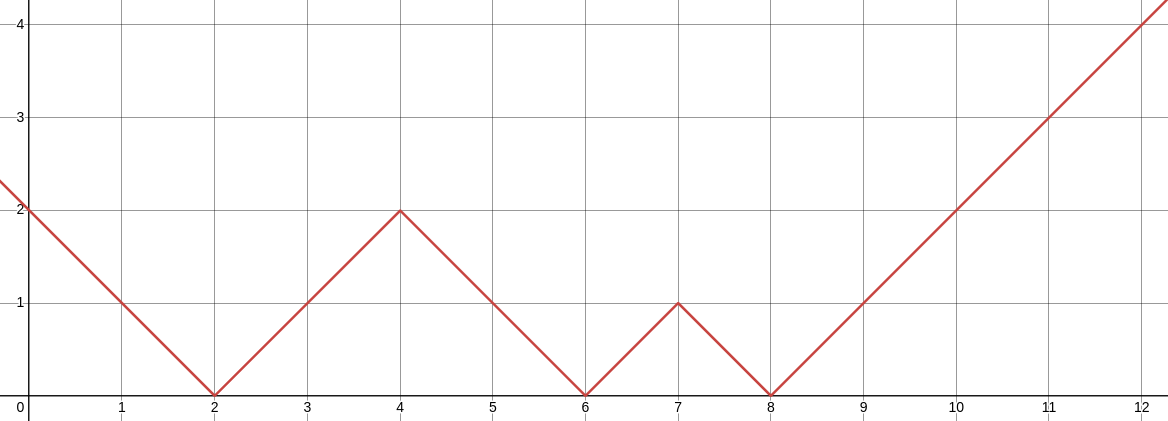
\includegraphics[width=0.75\linewidth]{img/absolute-0e.png}
\end{center}

Bob would like to create a mountain range by defining the function $A(x)$ using his favorite integer sequence $a_1, a_2, a_3, \dots, a_n$.  His painting will span from $x=0$ to $x=r$, and he will use green paint to shade in the region between $A(x)$ and the $x$-axis.

For example, if $a = [3, 1, 4, 1]$ and $r=6$, then the Bob would want to paint green the highlighted region in the diagram below.
\begin{center}
    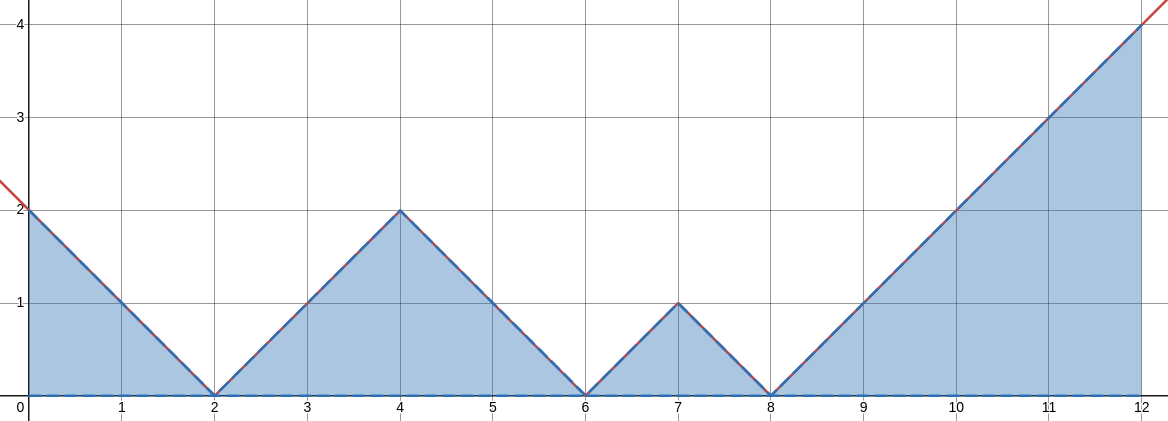
\includegraphics[width=0.75\linewidth]{img/absolute-1e.png}
\end{center}
Its total area can be shown to be \texttt{15} exactly.  In fact, Bob is able to show that if the $a_i$ are all even, then the area of the desired region is \textbf{guaranteed} to be an integer!

Given all these values, please determine the total \textit{area} of this region, so that Bob knows how much paint to buy.  It's \textit{integral} that he knows this information, \textit{definitely}!

\newpage

\subsection*{Input Format}

Input begins with a single line containing the space-separated integers $n$ and $r$.

The second line of input contains the $n$ space-separated integers $a_1, a_2, a_3, \dots, a_n$.

\subsection*{Output Format}

Output a line containing a single real number, the area of the desired region (rounded to exactly two decimal places).

\subsection*{Constraints}

\textit{Your program will only be tested on data that satisfies the following constraints.}

% Set to (10^5, 10^9) in true bounds
\constraints{
    $1 \leq n \leq 100$ \\
    $1 \leq r \leq 1000$ \\
}

\textit{There is no need to validate in your program that these constraints hold.}

\subsection*{Sample I/O}

\begin{sampleIO}
\begin{verbatim}
4 6
3 1 4 1
\end{verbatim}
&
\begin{verbatim}
3.75
\end{verbatim}
\end{sampleIO}

\begin{sampleIO}
\begin{verbatim}
1 2
1
\end{verbatim}
&
\begin{verbatim}
1.00
\end{verbatim}
\end{sampleIO}


% \subsection*{Explanation}

\cleardoublepage\relax% Slug: four-of-diamonds
% Description: ?
% Author: Cisco
% Story: Cisco
% Test Data: Cisco
% Testers: ?
% Editorial: ?
% TempSlug: four-of-diamonds

% Please don't modify or delete TempSlug

\problem{Kabayos!}
\begin{center}
    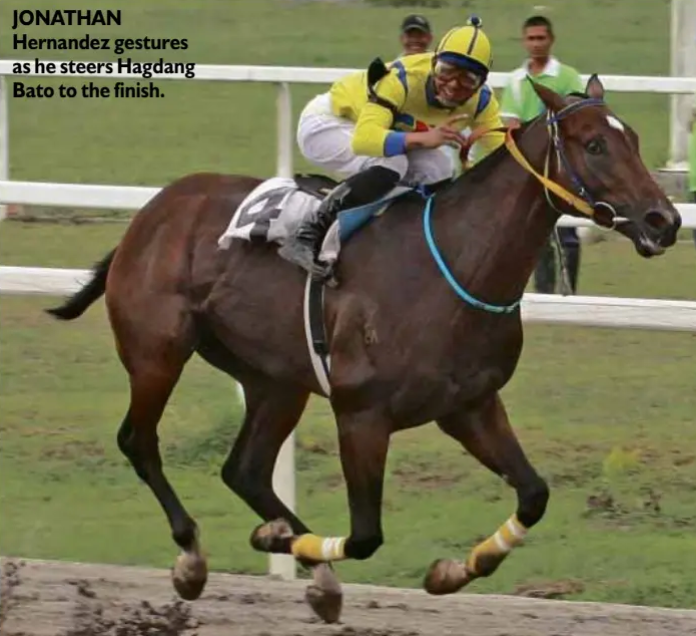
\includegraphics[width=0.4\linewidth]{img/hagdang-bato.png}

    \textit{2012 Philippine Triple Crown winner \textup{Hagdang Bato}, with his jockey JB Hernandez.}

    \textit{Image taken from the Philippine Daily Inquirer}
\end{center}

Cindy is addicted to a brand new horse-racing \textit{gacha} mobile game. The game is a \textit{raising simulator}, meaning the main gameplay loop is the process of training a character.  In this game, each of your characters is a \textit{kabayo}.

Each kabayo has $n$ attributes called ``stats'', each with some positive integer value.  There exists a \textit{stat cap} of $c$, meaning $c$ is the maximum value that any stat can be.

When one playthrough of the game is completed, Cindy's kabayo is assigned a numerical rating that is computed based on its stats, the higher the better.  

However, the rating formula is not linear.  The rating is computed as the \textit{sum of the squares} of each of Alice's kabayo's stats.  For example, with $n=5$, a kabayo with stats $[3, 1, 4, 1, 5]$ would have a rating of
\begin{align*}
    3^2 + 1^2 + 4^2 + 1^2 + 5^2 &= 52.
\end{align*}
Cindy's kabayo begins with some initial stats.  She then will decide how to train her kabayo, meaning she may do the following action at most $k$ times:
\begin{itemize}
    \item Choose one of her kabayo's stats with a value strictly less than $c$; \newline increase its value by $+1$.
\end{itemize}
You are given the initial stats of Cindy's kabayo, as well as $c$ and $k$.  If she raises her kabayo optimally, what is the maximum possible rating she can get?

\subsection*{Input Format}

Input begins with a single line containing the space-separated integers $n$ and $c$ and $k$.

The second line of input contains $n$ space-separated integers, the initial values of Cindy's kabayo's stats.

\subsection*{Output Format}

Output a line containing a single integer, the maximum possible rating.

\subsection*{Constraints}

\textit{Your program will only be tested on data that satisfies the following constraints.}

% Set to (2e5, 1e9, 1e6) in true bounds
\constraints{
    $1 \leq n \leq 100$ \\
    $1 \leq k \leq 2000$ \\
    $1 \leq c \leq 1200$ \\
    $1 \leq \text{each initial stat} \leq c$ \\
}

\textit{There is no need to validate in your program that these constraints hold.}

\subsection*{Sample I/O}

\begin{sampleIO}
\begin{verbatim}
5 6 2
3 1 4 1 5
\end{verbatim}
&
\begin{verbatim}
72
\end{verbatim}
\end{sampleIO}

\begin{sampleIO}
\begin{verbatim}
5 6 1
3 1 4 1 5
\end{verbatim}
&
\begin{verbatim}
63
\end{verbatim}
\end{sampleIO}

\begin{sampleIO}
\begin{verbatim}
5 5 1
3 1 4 1 5
\end{verbatim}
&
\begin{verbatim}
61
\end{verbatim}
\end{sampleIO}

\begin{sampleIO}
\begin{verbatim}
1 1200 99
1
\end{verbatim}
&
\begin{verbatim}
10000
\end{verbatim}
\end{sampleIO}

% \subsection*{Explanation}

\cleardoublepage\relax% Slug: four-of-diamonds
% Description: ?
% Author: Cisco
% Story: Cisco
% Test Data: Cisco
% Testers: ?
% Editorial: ?
% TempSlug: four-of-diamonds

% Please don't modify or delete TempSlug

\problem{Light Game}

Alice is replaying one of her favorite childhood platformers, \textit{Spongeboy: Skirmish for Scarborough Shoal}.  In this game, Spongeboy must defend his home from a ``robot'' invasion.  \textit{Supposedly}, it's said that the robots are an allegory for something, but Alice isn't quite sure what...  Metaphors are hard to decipher!

Aside from the main story, there are many puzzles which serve as side-objectives which can be completed for additional rewards.  One of these is the infamous \textit{Light Game}.

Spongeboy is dropped into a circular room, with $n$ lights arranged in sequence along the wall.  The lights are numbered $1$ to $n$ in the clockwise direction, and each light exists in one of two states: \textit{off} or \textit{on}. More formally, for each $1 \leq i \leq n$,
\begin{itemize}
\item for each $1 < i \leq n$, light $i-1$ is the left neighbor of light $i$ 
\newline (also, light $n$ is the left neighbor of light $1$);
\item for each $1 \leq i < n$, light $i+1$ is the right neighbor of light $i$ 
\newline (also, light $1$ is the right neighbor of light $n$).
\end{itemize}

Here is an example layout of the room with $n=8$.  Lights $3$ and $5$ and $7$ are initially on.
\begin{center}
    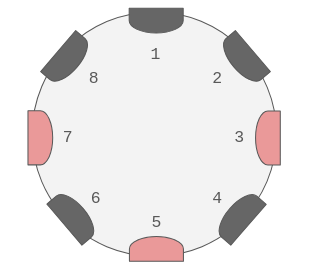
\includegraphics[width=0.3\linewidth]{img/light-game.png}
\end{center}


Each light is also a button that you can press.  When you press a light, the states of it and/or its neighbors may change, according to some seemingly random behavior.

Alice has a keen eye though, and deduced that the lights' behavior follows these consistent (if peculiar) rules:
\begin{itemize}
\item If you press a light where both its neighbors are off,
\newline both its neighbors are turned on
\item If you press a light where both its neighbors are on,
\newline its state is flipped \textit{and} both its neighbors are turned off.
\item If the pressed light has the same state as its left neighbor but not its right,
\newline the states of its two neighbors are \textit{both} flipped.
\item If the pressed light has the same state as its right neighbor but not its left,
\newline the state of the pressed light changes to be the same as its \textit{left} neighbor.
\end{itemize}
Here, ``flipping a state'' means: off lights become on, and on lights become off.

\newpage

Following the same example setup of $n=8$ lights from earlier (where initially, lights $3$ and $5$ and $7$ are on): if we press light $3$, then light $4$, then light $1$, then light $7$, we get the sequence of state changes illustrated in the diagram below.
\begin{center}
    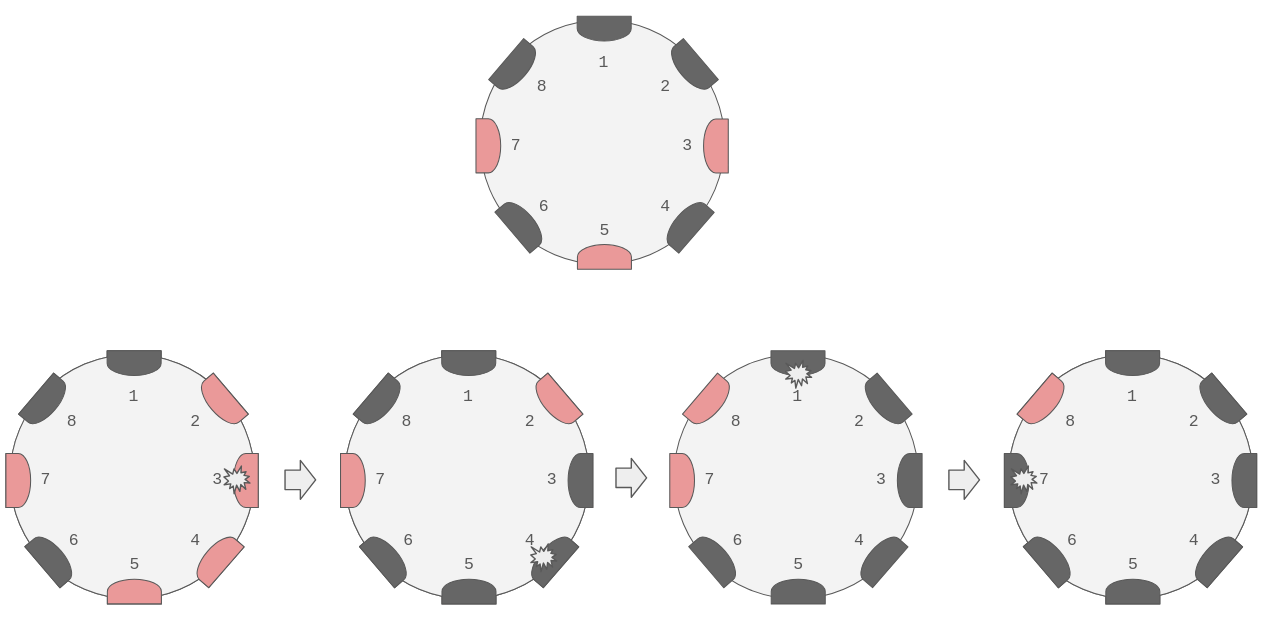
\includegraphics[width=0.85\linewidth]{img/light-press.png}

    \textit{We press light $3$, then press light $4$, then press light $1$, then press light $7$.}
\end{center}

You are given an initial configuration of lights, as well as the target configuration that Spongeboy must reach.  Does there exist \textit{any} sequence of button presses which achieves this goal?  If yes, please also construct such a solution.

\subsection*{Input Format}

Input consists of two lines, each containin a string of $n$ characters.  The first line represents the initial configuration, and the second line represents the target configuration.

The $i$th character is \texttt{1} if light $i$ is (or must be) on, and \texttt{0} if it is (or must be) off.  You are reminded that the room is \textit{circular}---despite the appearance of the input format, the first and last lights are actually next to each other.

\subsection*{Output Format}

Output a line containing \texttt{YES} if possible, and \texttt{NO} if not.

Then, if \texttt{YES}, output a solution.  First, output a line containing a non-negative integer $m$, the number of button presses in your construction.  Then, if $m > 0$, output another line containing $m$ space-separated integers, where each integer is from $1$ to $n$.  This encodes the instructions of which lights should be pressed, to be done in the order they are given.

Your solution must satisfy $m \leq 3 \cdot 10^5$.  Given the constraints, it can be shown that if a solution exists, then one satisfying $m \leq 3 \cdot 10^5$ exists.  If there are multiple possible answers, any will be accepted.

\newpage

\subsection*{Constraints}

\textit{Your program will only be tested on data that satisfies the following constraints.}

% Set to 10^5 in true bounds
\constraints{
    $3 \leq n \leq 100$ \\
    The input strings consist of \texttt{0} and \texttt{1} only.  \\
}

\textit{There is no need to validate in your program that these constraints hold.}

\subsection*{Sample I/O}

\begin{sampleIO}
\begin{verbatim}
00101010
00000001
\end{verbatim}
&
\begin{verbatim}
YES
4
3 4 1 7
\end{verbatim}
\end{sampleIO}

\begin{sampleIO}
\begin{verbatim}
000
111
\end{verbatim}
&
\begin{verbatim}
YES
3
3 3 3
\end{verbatim}
\end{sampleIO}


\begin{sampleIO}
\begin{verbatim}
01010
01010
\end{verbatim}
&
\begin{verbatim}
YES
0
\end{verbatim}
\end{sampleIO}


% \subsection*{Explanation}

\cleardoublepage\relax% Slug: four-of-diamonds
% Description: ?
% Author: Cisco
% Story: Cisco
% Test Data: Cisco
% Testers: ?
% Editorial: ?
% TempSlug: four-of-diamonds

% Please don't modify or delete TempSlug

\problem{Love Game}
\textit{Says Luna} (translated as \textit{Ani Buwan}) is a video game under the genre of \textit{dating simulator}.  You play the role of a young man who has inherited his grandfather's old farm, tasked with both adapting to rural life and forming bonds with your new community.

People in the community have an \textit{affection rating} for you, represented as some integer, possibly zero or negative (where negative affection corresponds to disdain).  Affection ratings are modified by giving these characters gifts.

Cindy is playing the game, and wants to reach an affection rating of $t$ or more with her favorite \textit{husbando}.  This husbando initially has an affection rating of $s$.  

However, at this stage of the game, Cindy only has access to one kind of item, the \textit{Square Seed}.  If she gives one Square Seed to her husbando, it has the following effect on his affection rating:
\begin{itemize}
    \item If his affection rating is currently $x$, then after receiving one Square Seed, \newline it becomes $x^2 - 3$.
\end{itemize}
So for example, if $s=-4$, then after giving the husbando one Square Seed, his affection rating becomes $13$.  After giving him another Square Seed, his affection rating then becomes $166$.

Given $s$ and $t$, determine the minimum number of Square Seeds Cindy must give her husbando in order for his affection rating to become $\geq t$.  If this is a fool's errand though (i.e. impossible no matter how many square seeds you give him), please tell Cindy.

\subsection*{Input Format}

Input consists of a single line containing the two space-separated integers $s$ and $t$.

\subsection*{Output Format}

If the task is impossible even if Cindy had all the Square Seeds in the world, output the words ``\texttt{MOVE ON}'' (without the quotes).

Otherwise, output a single non-negative integer, the minimum number of Square Seeds that Cindy needs to give her husbando.

\subsection*{Constraints}

\textit{Your program will only be tested on data that satisfies the following constraints.}

\constraints{
    $-10^9 \leq s, t \leq 10^9$ \\
}

\textit{There is no need to validate in your program that these constraints hold.}

\subsection*{Sample I/O}

\begin{sampleIO}
\begin{verbatim}
-4 100
\end{verbatim}
&
\begin{verbatim}
2
\end{verbatim}
\end{sampleIO}

\begin{sampleIO}
\begin{verbatim}
-99 -100
\end{verbatim}
&
\begin{verbatim}
0
\end{verbatim}
\end{sampleIO}

\begin{sampleIO}
\begin{verbatim}
0 1000
\end{verbatim}
&
\begin{verbatim}
4
\end{verbatim}
\end{sampleIO}



% \subsection*{Explanation}
% In the first sample input, the sequence already has the desired property.  The first \texttt{T} was the last tetromino of the previous bag.  Then, the next bag had the tetrominos in the order \texttt{OIJSZLT}.  Finally, the last \texttt{T} was the first tetromino of the next bag.

% In the second sample input, we can make the sequence have the desired property by, for example, changing the last two letters to \texttt{I} and \texttt{O}.
\cleardoublepage\relax% Slug: four-of-diamonds
% Description: ?
% Author: Cisco
% Story: Cisco
% Test Data: Cisco
% Testers: ?
% Editorial: ?
% TempSlug: four-of-diamonds

% Please don't modify or delete TempSlug

\problem{Mixed Messages}
I have a puzzle for you!  Can you decipher the hidden meaning in the following message?
\begin{center}
    \texttt{4427777}
\end{center}
This is a classic cipher.  Here's a hint:
\begin{center}
    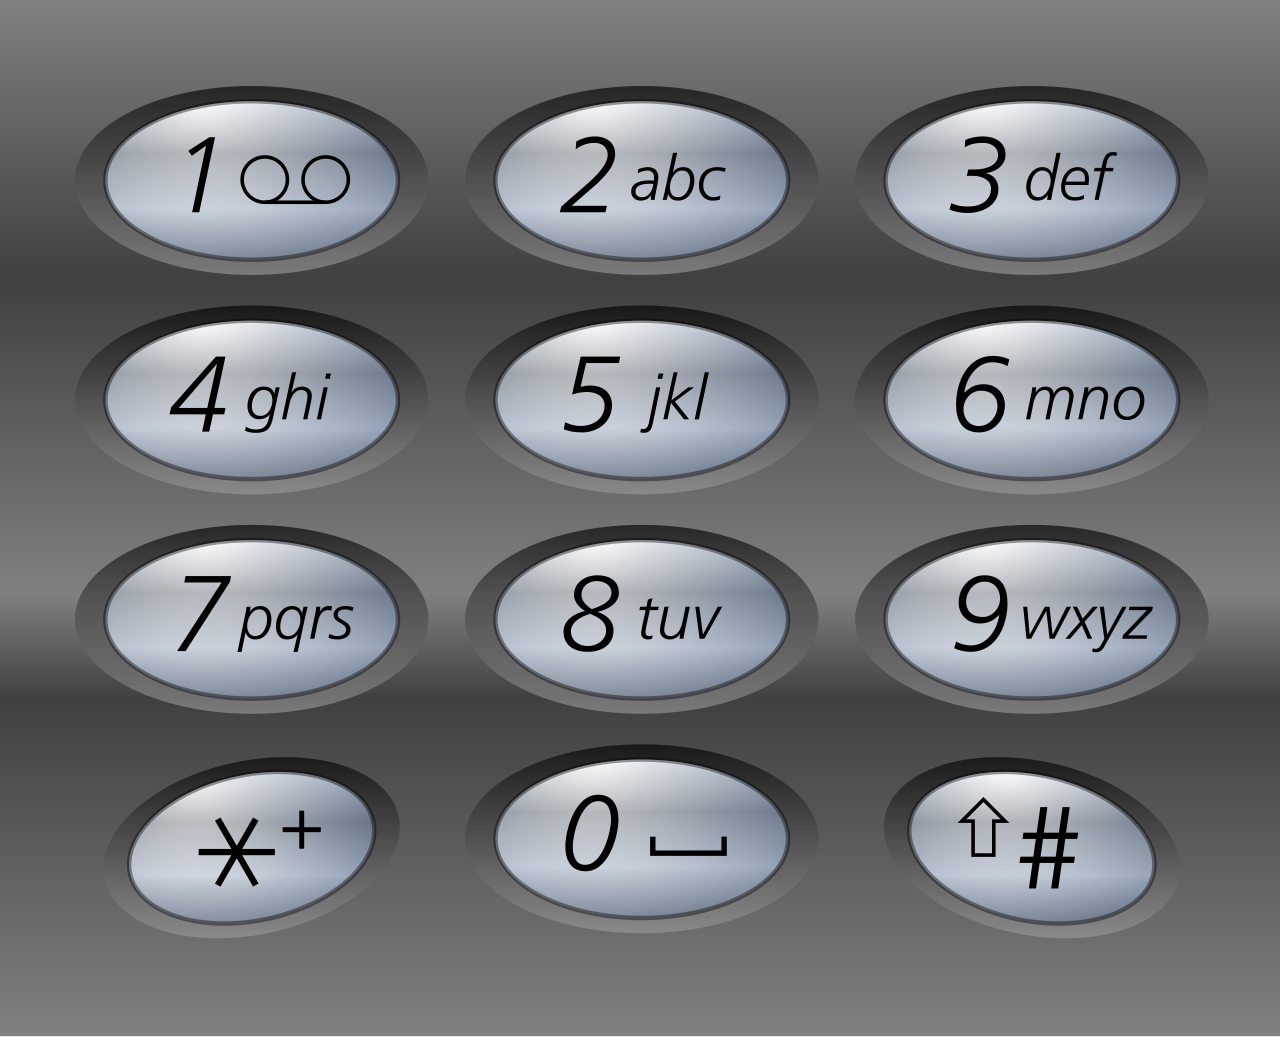
\includegraphics[width=0.25\linewidth]{img/keypad.png}

    \textit{Image taken from Wikipedia}
\end{center}
On an old cellphone keypad, letters are typed by pressing the corresponding key some number of times.  Each key is responsible for multiple letters (in the order they are written on the keypad), and each tap of the key would let you \textit{cycle} through your options which letter gets typed in.

For example, tapping \texttt{2} once would encode \texttt{a}, tapping it twice would encode \texttt{b}, and tapping it thrice would encode \texttt{c}.  One would ``lock in'' a choice by pausing before tapping again (usually you would have to wait for around one second between inputs).

We can use this to create a simple cipher.  Replace each English letter with the corresponding digit of the key it belongs to, repeated a number of times equal to the number of times you would tap that digit to get that letter.

For example, to translate the string \texttt{has}, we note that: \texttt{h} is \texttt{44}; \texttt{a} is \texttt{2}; and \texttt{s} is \texttt{7777}.  Concatenating them, we see that \texttt{has} is \texttt{4427777}.

The issue with this scheme is that by not encoding the pauses, it is posisble to have multiple words that map to the same ciphertext, making the message ambiguous.

For example, to translate the string \texttt{harp}, we note that: \texttt{h} is \texttt{44}; \texttt{a} is \texttt{2}; \texttt{r} is \texttt{777}; \newline and \texttt{p} is \texttt{7}.  Concatenating them, we see that \texttt{harp} is \textit{also} \texttt{4427777}.

Given a string of digits (each from \texttt{2} to \texttt{9}) to be interpreted as ciphertext, determine if the message is clear (if there is exactly one plaintext string which produces that ciphertext) or ambiguous (if multiple possible plaintext strings are encoded as that ciphertext).  \newline If the message is clear, please decode it for us as well!

\newpage

\subsection*{Input Format}

Input consists of a single line containing a string of digits (each from \texttt{2} to \texttt{9}), the ciphertext.

\subsection*{Output Format}

First, output a line containing either the string \texttt{CLEAR} or \texttt{AMBIGUOUS} according to the uniqueness of how to decode the ciphertext.

If \texttt{CLEAR}, also output another line containing the unique decrypted message (in all-lowercase letters).

\subsection*{Constraints}

\textit{Your program will only be tested on data that satisfies the following constraints.}

% Set to 10^5 in true bounds
\constraints{
    The ciphertext consists of at least $1$ and at most $100$ digits, each from \texttt{2} to \texttt{9}.\\
}

\textit{There is no need to validate in your program that these constraints hold.}

\subsection*{Sample I/O}

\begin{sampleIO}
\begin{verbatim}
725262
\end{verbatim}
&
\begin{verbatim}
CLEAR
pajama
\end{verbatim}
\end{sampleIO}

\begin{sampleIO}
\begin{verbatim}
4427777
\end{verbatim}
&
\begin{verbatim}
AMBIGUOUS
\end{verbatim}
\end{sampleIO}


% \subsection*{Explanation}

\cleardoublepage\relax% Slug: four-of-diamonds
% Description: ?
% Author: Cisco
% Story: Cisco
% Test Data: Cisco
% Testers: ?
% Editorial: ?
% TempSlug: four-of-diamonds

% Please don't modify or delete TempSlug

\problem{Six Seven}
Alice was tasked with implementing Dijkstra's shunting yard, an algorithm for parsing arithmetic expressions, respecting correct operator precedence (i.e. MDAS).  However, she submitted a meme instead, which annoyed her teacher.
\begin{itemize}
    \item The \texttt{+} operation is implemented as \textbf{string concatenation} instead of addition, \newline e.g. \texttt{6 + 7} evaluates to \texttt{67}
    \item The \texttt{*} operation is implemented as \textbf{string duplication} instead of multiplication, \newline e.g. \texttt{6 * 7} evaluates to \texttt{6666666}
    \item The \texttt{-} operation is implemented as normal, except negative numbers were not implemented, so if any operation would result in one at any intermediate step \newline (e.g. \texttt{6 - 7}) then the computer explodes.
    \item The \texttt{/} operation is implemented as normal, except non-integer fractions were not implemented, so if any operation would result in one at any intermediate step \newline (e.g. \texttt{6 / 7}) then the computer explodes.
    \item Finally, the \textbf{only} accepted integer literals are \texttt{6} and \texttt{7}.
\end{itemize}
Otherwise, her program correctly follows the MDAS convention.
\begin{itemize}
    \item It recursively evaluates parenthesized expressions first, then
    \item resolves \texttt{*} and \texttt{/} operations from left to right, then
    \item resolves \texttt{+} and \texttt{-} operations from left to right.
\end{itemize}
Alice's program ignores spaces between tokens.

For example, \texttt{7 - 6 + 6} equals \texttt{16}, evaluated as follows:
\begin{align*}
    \texttt{7 - 6 + 6}
    &= \texttt{{\color{red}1} + 6} \\
    &= \texttt{{\color{red}16}}.
\end{align*}

For another example, \texttt{(7+7) - (6+7 - 7)/6} equals \texttt{67}, evaluated as follows:
\begin{align*}
    \texttt{(7+7) - (6+7 - 7)/6}
    &= \texttt{{\color{red}77} - (6+7 - 7)/6}, \\
    &= \texttt{77 - ({\color{red}67} - 7)/6}, \\
    &= \texttt{77 - {\color{red}60}/6}, \\
    &= \texttt{77 - \color{red}10} \\
    &= \texttt{\color{red}67}.
\end{align*}

For one final example, \texttt{6*6 / (6 + (6 + 6)) / 7} equals \texttt{143}, evaluated as follows:
\begin{align*}
    \texttt{6*6 / (6 + (6 + 6)) / 7}
    &= \texttt{6*6 / (6 + {\color{red}66}) / 7} \\
    &= \texttt{6*6 / {\color{red}666} / 7} \\
    &= \texttt{{\color{red}666666} / 666 / 7} \\
    &= \texttt{{\color{red}1001} / 7} \\
    &= \texttt{{\color{red}143}}.
\end{align*}

Given a positive integer $n$, your goal is to construct any arithmetic expression (using parentheses, \texttt{6} and \texttt{7}, and the \texttt{*/+-} operations) which evaluates to $n$ using Alice's meme program.  \textit{For completeness}, here are the other limitations of Alice's program:
\begin{itemize}
    \item If the expression contains more than $1000$ characters (including spaces), \newline the computer blows up.
    \item If at any intermediate step an integer with a value greater than $2^{64}$ is produced, \newline the computer blows up.
    \item For \texttt{+} and \texttt{*}, leading zeros are removed at each intermediate step, \newline e.g. \texttt{0 + 0} and \texttt{0 * 5} both evaluate to \texttt{0} (just one \texttt{0})
    \item Finally, \texttt{n * 0} causes the computer to blow up, regardless of the left operand.
\end{itemize}

\subsection*{Input Format}

Input consists of a single positive integer $n$.


\subsection*{Output Format}

Output a single line containing \textit{any} valid expression which evaluates to $n$.

We give the following formal definition of what exactly constitutes an \textit{expression}.

An \textit{expression} is a sequence of one or more sub-expressions, separated by operators.  \newline
A \textit{sub-expression} is one of the following:
\begin{itemize}
\item an integer literal (which must be \texttt{6} or \texttt{7}); or
\item another expression, enclosed in parentheses \texttt{()}
\end{itemize}

Each operator must be one of \texttt{+} or \texttt{-} or \texttt{*} or \texttt{/}

Spaces between tokens are ignored, so add as many as you like (within the char. count).

Here are some more examples of valid expressions:
\begin{center}
    \texttt{(7) - ((6)) + (((7)))}
    
    \texttt{(6 + 7 * 6)}

    \texttt{(6 / 6) * (7)}

    \texttt{(((((((6)))))))}

    \texttt{7}
\end{center}
These evaluate to \texttt{17} and \texttt{6777777} and \texttt{1111111} and \texttt{6} and \texttt{7}, respectively.

\subsection*{Constraints}

\textit{Your program will only be tested on data that satisfies the following constraints.}

\constraints{
    $1 \leq n \leq 10^{12}$ \\
}

\textit{There is no need to validate in your program that these constraints hold.}

% \newpage

\subsection*{Sample I/O}

\begin{sampleIO}
\begin{verbatim}
16
\end{verbatim}
&
\begin{verbatim}
7 - 6 + 6
\end{verbatim}
\end{sampleIO}

\begin{sampleIO}
\begin{verbatim}
67
\end{verbatim}
&
\begin{verbatim}
(7+7) - (6+7 - 7)/6
\end{verbatim}
\end{sampleIO}


\begin{sampleIO}
\begin{verbatim}
143
\end{verbatim}
&
\begin{verbatim}
6*6 / (6 + (6 + 6)) / 7
\end{verbatim}
\end{sampleIO}


\begin{sampleIO}
\begin{verbatim}
17
\end{verbatim}
&
\begin{verbatim}
(7) - ((6)) + (((7)))
\end{verbatim}
\end{sampleIO}


\begin{sampleIO}
\begin{verbatim}
6777777
\end{verbatim}
&
\begin{verbatim}
(6 + 7 * 6)
\end{verbatim}
\end{sampleIO}


\begin{sampleIO}
\begin{verbatim}
1111111
\end{verbatim}
&
\begin{verbatim}
(6 / 6) * (7)
\end{verbatim}
\end{sampleIO}



\begin{sampleIO}
\begin{verbatim}
6
\end{verbatim}
&
\begin{verbatim}
(((((((6)))))))
\end{verbatim}
\end{sampleIO}



\begin{sampleIO}
\begin{verbatim}
7
\end{verbatim}
&
\begin{verbatim}
7
\end{verbatim}
\end{sampleIO}



% \subsection*{Explanation}
% TODO
\cleardoublepage\relax% Slug: four-of-diamonds
% Description: ?
% Author: Cisco
% Story: Cisco
% Test Data: Cisco
% Testers: ?
% Editorial: ?
% TempSlug: four-of-diamonds

% Please don't modify or delete TempSlug

\problem{Tetris Fanfiction}
A \textit{tetromino} is a shape formed by connecting four unit squares together edge-to-edge.  If we count rotations as fundamentally the same shape (but reflections are distinct!), then there are \textit{seven} different tetrominos, illustrated below.  Each is commonly associated with an uppercase English letter whose shape it resembles.
\begin{center}
    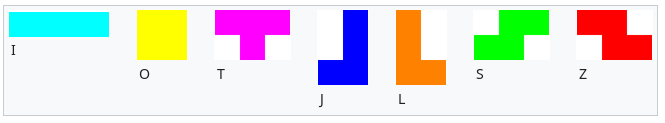
\includegraphics[width=0.75\linewidth]{img/tetris.png}

    \textit{Image taken from Wikipedia}
\end{center}

Tetris is a game in which you are randomly given tetrominos one at a time, and must place them onto to the gameboard in the order you receive them.

Did you know that each next tetris piece is not generated independently from the others?  The sequence of tetris pieces is generated according to the ``7-bag'' algorithm described as follows.  Begin with an empty sequence, then repeat this infinitely many times:
\begin{itemize}
    \item Among all possible permutations of the seven tetrominos, select one of them uniformly at random (this is a ``7-bag'').
    \item Then, append these seven tetrominos \textit{in that random order} as the next seven terms of the sequence.
\end{itemize}
This ensures that there will never be ``droughts'' or ``floods'' of a particular piece, along with many other desirable mathematical properties.

For example, the first sixteen tetrominos in a Tetris game might look like this.  For illustration, tetrominos belonging to the same 7-bag are shown grouped together.
\begin{center}
    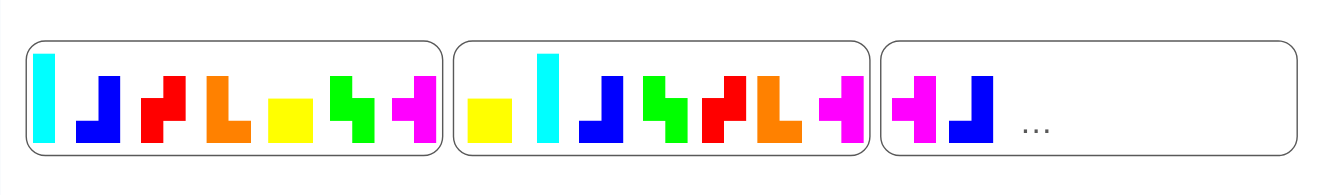
\includegraphics[width=0.95\linewidth]{img/tetris-bag.png}
\end{center}

Bob is writing some Tetris fanfiction, and wants to include the following scene:
\begin{itemize}
    \item \textit{Tetra started a game of Tetris and played for some unknown amount of time.  She paused the game.  Then, when she resumed, we observed that the pieces she got were $t_1$, then $t_2$, then $t_3$, and so on, until $t_n$.}
\end{itemize}
Bob cares about his story being accurate to the game mechanics of real life Tetris.  Is it possible for the sequence $t_1, t_2, t_3, \dots, t_n$ to appear consecutively somewhere in some sequence generated by the 7-bag algorithm?  And if not, what is the fewest number of terms that need to be changed in order to make it so?

\newpage

\subsection*{Input Format}

Input consists of a single line containing a string of $n$ uppercase English letters, each one of \texttt{IJLOSTZ}, where the $i$th letter in the string identifies the tetromino $t_i$.

\subsection*{Output Format}

Output a single integer, the fewest number of terms that need to be changed in order for Bob's sequence to have the desired property.  Note that if it already does have the desired property, you should output $0$.

\subsection*{Constraints}

\textit{Your program will only be tested on data that satisfies the following constraints.}

% Set to 10^5 in true bounds
\constraints{
    $1 \leq n \leq 100$ \\
    Each letter is one of \texttt{IJLOSTZ} \\
}

\textit{There is no need to validate in your program that these constraints hold.}

\subsection*{Sample I/O}

\begin{sampleIO}
\begin{verbatim}
TOIJSZLTT
\end{verbatim}
&
\begin{verbatim}
0
\end{verbatim}
\end{sampleIO}

\begin{sampleIO}
\begin{verbatim}
ZZZZ
\end{verbatim}
&
\begin{verbatim}
2
\end{verbatim}
\end{sampleIO}

\begin{sampleIO}
\begin{verbatim}
TILLJOLTLILTLOSTZITI
\end{verbatim}
&
\begin{verbatim}
4
\end{verbatim}
\end{sampleIO}



\subsection*{Explanation}
In the first sample input, the sequence already has the desired property.  The first \texttt{T} was the last tetromino of the previous bag.  Then, the next bag had the tetrominos in the order \texttt{OIJSZLT}.  Finally, the last \texttt{T} was the first tetromino of the next bag.

In the second sample input, we can make the sequence have the desired property by, for example, changing the last two letters to \texttt{I} and \texttt{O}.
\cleardoublepage\relax% Slug: four-of-diamonds
% Description: ?
% Author: Cisco
% Story: Cisco
% Test Data: Cisco
% Testers: ?
% Editorial: ?
% TempSlug: four-of-diamonds

% Please don't modify or delete TempSlug

\problem{The Parlor}
Herbert S. Sinclair is developing a suite of puzzles to challenge his grand-nephew Simon Jones, who will be visiting his manor within the coming months.  Each room in his manor has a distinct gimmick, and the style of puzzle to be placed in The Parlor is as follows.

There are three boxes of three different colors: blue, white, and black, laid out in a row in that order.  Each box has a statement written on it.
\begin{center}
    
\includegraphics[width=0.7\linewidth]{img/parlor-boxes.png}

    \textit{Image taken from PC Gamer}
\end{center}

In the room, one would find the following note, explaining the rules of the game:
\begin{center}
    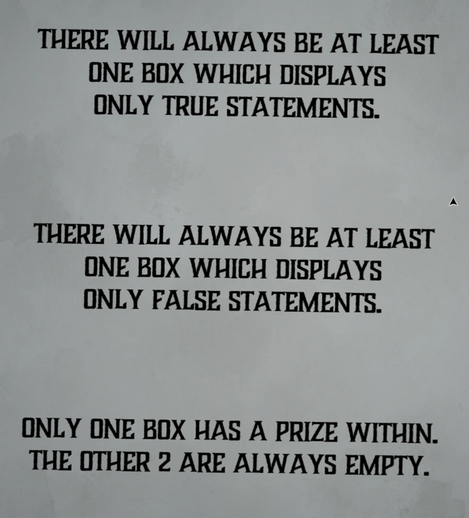
\includegraphics[width=0.3\linewidth]{img/parlor-notes.png}

    \textit{Image taken from the Blue Prince wikia}
\end{center}
Each statement in the room is of one of the following forms:

\begin{itemize}
    \item \texttt{The gems <'are' | 'are not'> in the <'blue' | 'white' | 'black'> box.}
    \item \texttt{The statement on the <'blue' | 'white' | 'black'> box is <'true' | 'false'>.}
    \item \texttt{The statement on the box with the gems is <'true' | 'false'>.}
    \item \texttt{The statements on the empty boxes are both <'true' | 'false'>.}
    \item \texttt{Exactly one box has a statement that is <'true' | 'false'>.}
    \item \texttt{Exactly two boxes have a statement that is <'true' | 'false'>.}
\end{itemize}

The gems, of course, are the prize.  Simon must deduce which box contains the gems.

You have been hired as a playtester for the parlor puzzle.  Given statements that would be placed on these boxes, determine if they have a unique solution, admit multiple solutions, or are paradoxical.  Additionally, if they admit a unique solution, determine which box contains the gems.

\subsection*{Input Format}

The first line of input contains a single integer $T$, the number of test cases.  Then, the descriptions of the $T$ test cases follow.

Each test case is described by four lines: the statement on the blue box, then the statement on the white box, then the statement on the black box, and finally a ``separator'' line consisting of the \texttt{-} character repeated $75$ times.


\subsection*{Output Format}

Output the answer to each test case in its own line.
\begin{itemize}
    \item If---according to the rules of the game---it should have been impossible for the boxes to display these statements, output \texttt{PARADOX}
    \item If the answer can be uniquely deduced from the statements (and the rules of the game), output the color of the box with the gems: one of \texttt{blue} or \texttt{white} or \texttt{black}
    \item If the given statements (and rules of the game) do not determine a unique answer, output \texttt{AMBIGUOUS} instead.
\end{itemize}

\subsection*{Constraints}

\textit{Your program will only be tested on data that satisfies the following constraints.}

% Set to 10^5 in true bounds
\constraints{
    $1 \leq T \leq 400$ \\
    Each statement exactly follows one of the above formats. \\
}

\textit{There is no need to validate in your program that these constraints hold.}

\subsection*{Sample I/O}

\begin{sampleIO}
\begin{verbatim}
TODO
\end{verbatim}
&
\begin{verbatim}
TODO
\end{verbatim}
\end{sampleIO}


\subsection*{Explanation}
Suppose the statement on the white box is false.
\begin{itemize}
\item This directly tells us that the statement on the blue box is false.
\item There must be a true statement, so the statement on the black box must be the true one.
\item Because the statement on the blue box is \textit{false}, we conclude that the gems are in a box with a true statement.
\item So, the gems are in the black box!
\item But... if the black box were true, then the gems \textit{should} be in the blue box.
\item This is a \textbf{contradiction}, so we conclude that the statement on the white box is true.
\end{itemize}

On the other hand, suppose the statement on the white box is true.
\begin{itemize}
\item This directly tells us that the statement on the blue box is true.
\item There must be a false statement, so the statement on the black box must be the false one.
\item Because the statement on the blue box is \textit{true}, we conclude that the gems are in a box with a false statement
\item The statement on the black box (that the gems are in the blue) was indeed false!
\end{itemize}


On the other hand suppose the statement 
\cleardoublepage\relax% Slug: four-of-diamonds
% Description: ?
% Author: Cisco
% Story: Cisco
% Test Data: Cisco
% Testers: ?
% Editorial: ?
% TempSlug: four-of-diamonds

% Please don't modify or delete TempSlug

\problem{The Rainbow Connection}
Alice, Bob, and Cindy are playing a co-op puzzle game called \textit{The Rainbow Connection}.

In one of the puzzles, there are four columns arranged in a row, each with $n$ nodes labeled $1$ to $n$ from top to bottom.  The spaces between the columns are labeled Zone A, Zone B, and Zone C from left to right.  Here is an illustration of the setup with $n=4$.
\begin{center}
    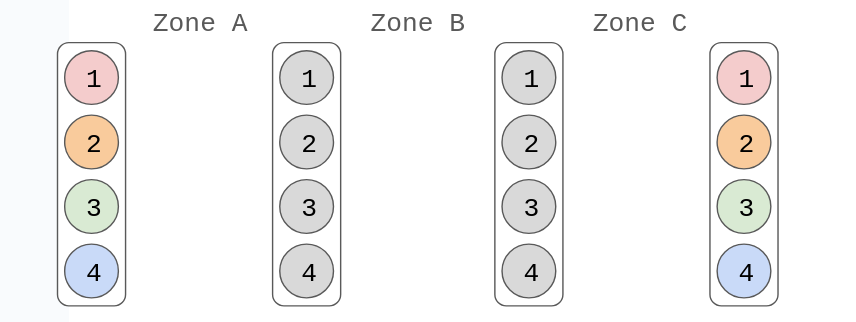
\includegraphics[width=0.575\linewidth]{img/rainbow-b.png}
\end{center}
In this game, you place wires in each of the zones, with each wire connecting a node on the left with some node on the right.

Alice and Cindy got a bit excited and immediately started drawing wires in Zones A and C respectively.  Alice drew $n$ wires, but made it so that there is no node connected to two wires; so did Cindy.  For example, with $n=4$, they might have done the following.
\begin{center}
    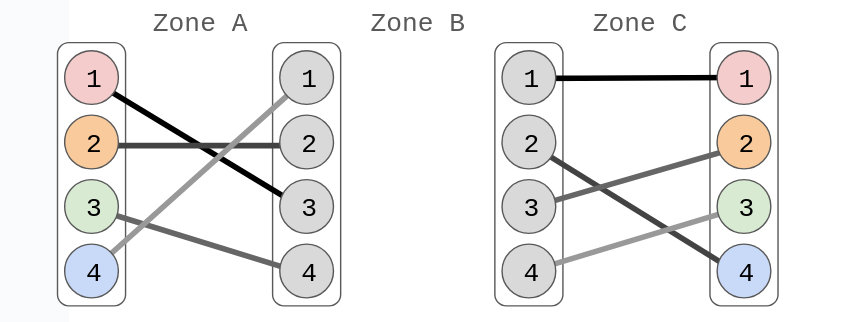
\includegraphics[width=0.575\linewidth]{img/rainbow-1-b.png}
\end{center}
Only after they did this did they read the rules.  They must draw wires such that, for each $i$ from $1$ to $n$: current emitted from the leftmost node $i$ will---if it follows the wires they've drawn---terminate on the rightmost node $i$.

Oops.  Oh well, Bob can still save them, right?  In the example from earlier, the task can still be completed if Bob draws his wires as follows.
\begin{center}
    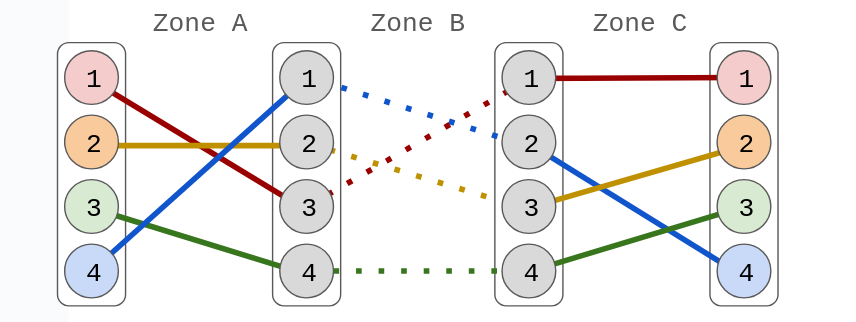
\includegraphics[width=0.575\linewidth]{img/rainbow-2-b.png}
\end{center}

Given the manner in which Alice and Cindy drew their wires, determine how Bob must draw his wires in order for the task to be completed.  It can be shown that the task is always possible.

\subsection*{Input Format}

The first line of input contains a single integer $n$.

The second line of input contains $n$ space-separated integers $a_1, a_2, \dots, a_n$, each a \textit{distinct} integer from $1$ to $n$.  This means that Alice connected node $i$ on her left with node $a_i$ on her right.

The third line of input contains $n$ space-separated integers $c_1, c_2, \dots, c_n$, each a \textit{distinct} integer from $1$ to $n$.  This means that Cindy connected node $i$ on her left with node $c_i$ on her right.

\subsection*{Output Format}

Output $n$ space-separated integers $b_1, b_2, \dots, b_n$, each a \textit{distinct} integer from $1$ to $n$.  This means that Bob will connect node $i$ on his left with node $b_i$ on his right.

If there are multiple possible answers, any will be accepted.

\subsection*{Constraints}

\textit{Your program will only be tested on data that satisfies the following constraints.}

% Set to 10^5 in true bounds
\constraints{
    $2 \leq n \leq 100$ \\
    $a_1, a_2, \dots, a_n$ are distinct integers from $1$ to $n$. \\
    $c_1, c_2, \dots, c_n$ are distinct integers from $1$ to $n$. \\
}

\textit{There is no need to validate in your program that these constraints hold.}

\subsection*{Sample I/O}

\begin{sampleIO}
\begin{verbatim}
4
3 2 4 1
1 4 2 3
\end{verbatim}
&
\begin{verbatim}
2 3 1 4
\end{verbatim}
\end{sampleIO}

\begin{sampleIO}
\begin{verbatim}
7
1 2 3 4 5 6 7
1 2 3 4 5 6 7
\end{verbatim}
&
\begin{verbatim}
1 2 3 4 5 6 7
\end{verbatim}
\end{sampleIO}


% \subsection*{Explanation}
% TODO
\end{document}
